
\documentclass[11pt,fleqn]{article} 
\usepackage[margin=0.8in, head=0.8in]{geometry} 
\usepackage{amsmath, amssymb, amsthm}
\usepackage{fancyhdr} 
\usepackage{palatino, url, multicol}
\usepackage{graphicx, pgfplots} 
\usepackage[all]{xy}
\usepackage{polynom} 
%\usepackage{pdfsync} %% I don't know why this messes up tabular column widths
\usepackage{enumerate}
\usepackage{framed}
\usepackage{setspace}
\usepackage{array,tikz}

\pgfplotsset{compat=1.6}

\pgfplotsset{soldot/.style={color=black,only marks,mark=*}} \pgfplotsset{holdot/.style={color=black,fill=white,only marks,mark=*}}
\pgfplotsset{my style/.append style={axis x line=middle, axis y line=
middle, xlabel={$x$}, ylabel={$y$}, axis equal }}


\pagestyle{fancy} 
\lfoot{}
\rfoot{3-2 Derivative as Function}

\begin{document}
\renewcommand{\headrulewidth}{0pt}
\newcommand{\blank}[1]{\rule{#1}{0.75pt}}
\newcommand{\bc}{\begin{center}}
\newcommand{\ec}{\end{center}}
\renewcommand{\d}{\displaystyle}

\vspace*{-0.7in}

%%%%%%%%%intro page
\begin{center}
  \large
  \sc{Section 3-2: The Derivative as a Function}\\
\end{center}
\begin{enumerate}
\item Write the definition of $f'(x),$ the derivative of the function $f(x)$,\\
\vspace{.7in}
\item Let $f(x)=\sqrt{x+5}.$
\begin{enumerate}
	\item Use the definition of the derivative to find $f'(x).$
	\vspace{3in}
	\item Sketch $f(x)$ and $f'(x)$ on the same set of axes. (Use technology if you like.)
	\vspace{2in}
	\item Write the equation of the line tangent to $f(x)$ at $x=0.$
	\vspace{1in}
	\end{enumerate}

\item On the next page are several graphs. For each one, sketch the graph of $f'(x)$ on the axes below.
\newpage
\vspace*{-.5in}
\begin{tabular}[c]{c  c }

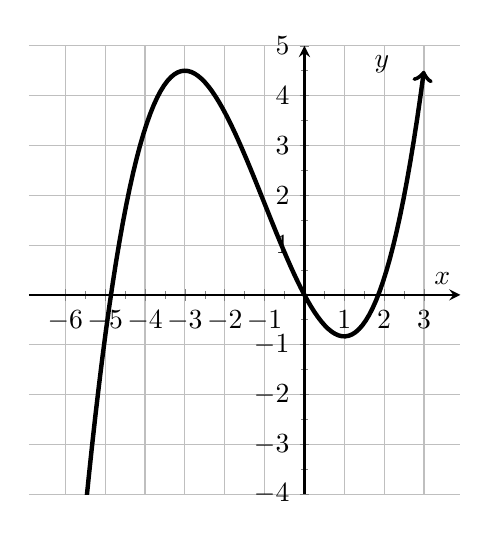
\begin{tikzpicture}
%cubic
\begin{axis}[xscale=.8, thick, my style, xtick={-6,-5,...,3}, ytick={-10,-9,...,10},xmin=-6, xmax=3, ymin=-4, ymax=5, minor y tick num=1, minor x tick num=1, 
mark size=3.0pt, grid = major]
\addplot[ultra thick, <->,domain=-5.5:3, samples=100]{-((3*x)/2) + x^2/2 + x^3/6};
\end{axis}
\end{tikzpicture}
&
%quartic
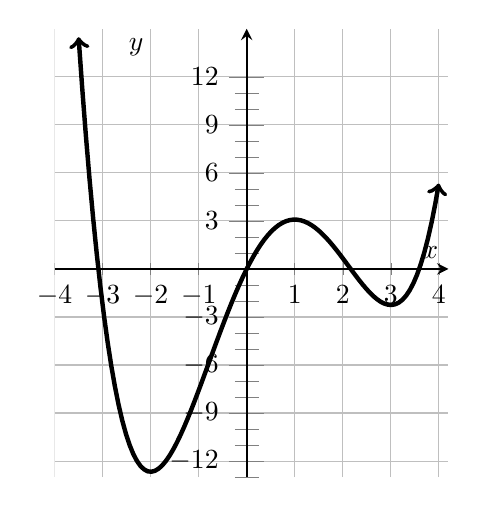
\begin{tikzpicture}
\begin{axis}[xscale=3, thick, my style, xtick={-4,-3,...,4}, ytick={-15,-12,...,12},
xmin=-4, xmax=4.2, 
ymin=-13, ymax=15, minor y tick num=2, minor x tick num=0, 
mark size=3.0pt, grid = major, axis equal image]
\addplot[ultra thick, <->,domain=-3.5:4, samples=100]{6*x - (5*x^2)/2 - (2*x^3)/3 + x^4/4};
\end{axis}
\end{tikzpicture}
\\
%below cubic
\begin{tikzpicture}
\begin{axis}[xscale=.8, thick, my style, xtick={-6,-5,...,3}, ytick=\empty,%ytick={-10,-9,...,10},
xmin=-6, xmax=3, ymin=-4, ymax=5, minor y tick num=1, minor x tick num=0, 
%mark size=3.0pt, axis equal image %grid = major
]
\end{axis}
\end{tikzpicture}
&
%below quartic
\begin{tikzpicture}
\begin{axis}[xscale=3, thick, my style, xtick={-4,-3,...,4}, ytick=\empty,
xmin=-4, xmax=4.2, 
ymin=-13, ymax=15, minor y tick num=0, minor x tick num=0, 
mark size=3.0pt, %grid = major, 
axis equal image]
\end{axis}
\end{tikzpicture}
\\
%piecewise
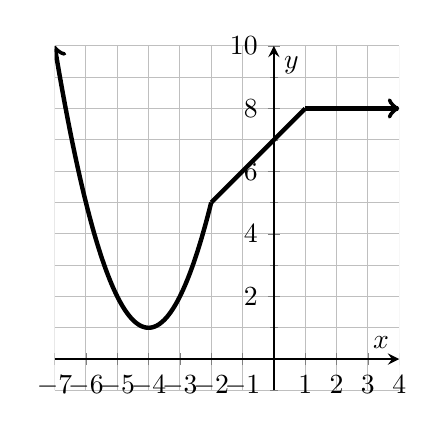
\begin{tikzpicture}
\begin{axis}[scale=1.2, thick, my style, xtick={-8,-7,...,4}, ytick={-4,-2,...,10},
xmin=-7, xmax=4, ymin=-1, ymax=10, minor y tick num=1,
        minor x tick num=0, mark size=3.0pt, grid = both, axis equal image, width=.5\linewidth]
        \addplot[ultra thick, <-,domain=-7:-2, samples=100]{1 + (4 + x)^2};
         \addplot[ultra thick,domain=-2:1, samples=100]{7+x};
         \addplot[ultra thick, ->,domain=1:4, samples=100]{8};
\end{axis}
\end{tikzpicture}
&
%x^1/3
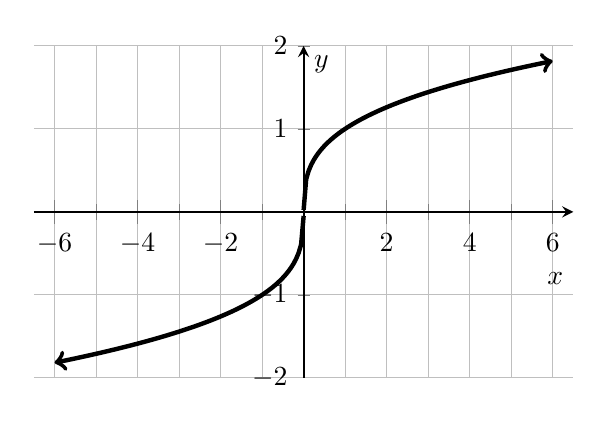
\begin{tikzpicture}
\begin{axis}[xscale = 1, yscale = 2, thick, my style, %xtick={-6,-5...,6}, ytick={-2,-1,...,2},
xmin=-6.5, xmax=6.5, ymin=-2, ymax=2, minor y tick num=0,
minor x tick num=1, 
mark size=3.0pt, grid = both, axis equal image,]
        \addplot[ultra thick, ->,domain=.00001:6, samples=100]{x^(1/3)};
       \addplot[ultra thick, <-,domain=-6:-.00001, samples=100]{ -(-x)^(1/3)};
\end{axis}
\end{tikzpicture}
\\
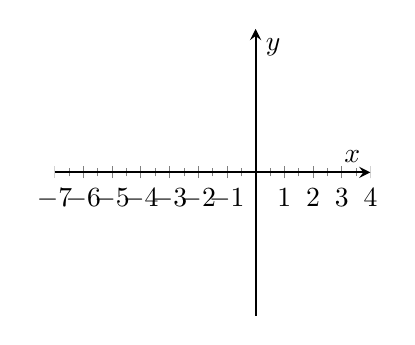
\begin{tikzpicture}
\begin{axis}[scale=1, thick, my style, xtick={-8,-7,...,4}, ytick=\empty,
xmin=-7, xmax=4, ymin=-5, ymax=5, minor y tick num=1,
        minor x tick num=1, mark size=3.0pt, %grid = both, 
        axis equal image, width=.5\linewidth]
\end{axis}
\end{tikzpicture}
&
\begin{tikzpicture}
\begin{axis}[xscale = 1, yscale = 2, thick, my style, %xtick={-6,-5...,6}, 
ytick=\empty,
xmin=-6.5, xmax=6.5, ymin=-3, ymax=3, minor y tick num=0,
minor x tick num=1, 
mark size=3.0pt, %grid = both, 
axis equal image,]
\end{axis}
\end{tikzpicture}


\end{tabular}
\end{enumerate}
\end{document}

